\newpage
%
%	Численное дифференцирование
%
\section{Численное дифференцирование}
Задача численного дифференцирования состоит 
в приближенном вычислении производных функции $y(x)$
по заданным в конечном числе точек $\{x_i\}$ 
значениям этой функции.

Численное дифференцирование применяется, 
если функцию $y(x)$ трудно или невозможно 
продифференцировать аналитически, например, если 
функция является таблично заданной, а также 
при решении дифференциальных уравнений 
разностными методами.

Многие формулы численного дифференцирования можно получить, 
используя интерполяционные формулы.
Для этого достаточно заменить функцию $y(x)$ 
интерполяционным полиномом Лагранжа $L_n(x)$ 
и вычислить производные этого многочлена, 
используя его явное представление.

Рассмотрим произвольную сетку $\{x_i\}$ и 
проведем интерполирование функции $y(x)$ в узлах сетки 
$x_{i-1} < x_{i} < x_{i+1}$ полиномом Лагранжа второго
порядка, приближенно полагая $y(x)\approx L_{2}(x)$
для $x\in[x_{i-1},x_{i+1}]$:
% *******************************
%	График функций
%
\begin{figure}[H]\centering
\begin{tikzpicture}
\begin{axis}[
%axis lines = middle,
every axis/.style={color=black, solid, thick},
xlabel = {\empty},		% подпись оси x
ylabel = {\empty},	% подпись оси y
xmin=-0.75, xmax=2,
ymin=-0.5, ymax=3,
%xtick style={thick, black}, 
xtick={-0.5,0,1.75}, xticklabels={$x_{i-1}$,$x_i$,$x_{i+1}$},
%ytick style={thick, black}, 
ytick={2.25,1,0.5625}, yticklabels={$y_{i-1}$,$y_i$,$y_{i+1}$},
grid=major,		
major grid style={color=black!20, dashed, thin},
]
\addplot [only marks,mark=ball,ball color=darkred!75,
mark size=4pt,mark options={draw=darkred,thin}]
coordinates {(-0.5,2.25) (0,1) (1.75,0.5625)};
\addplot [color=darkred, thick, domain=-0.5:1.75] 
{(x-1)^2} node[pos=0.75,above] {$L_2(x)$};
\end{axis}
\end{tikzpicture}
\end{figure}
% *******************************
\begin{equation*}
\label{approx2}
\begin{matrix}
L_{2}(x)
&=&\dfrac
{ (x-x_{i})\cdot(x-x_{i+1}) }
{ (x_{i-1}-x_{i})\cdot(x_{i-1}-x_{i+1}) } \cdot y_{i-1}& + \\
\\
&+&\dfrac
{ (x-x_{i-1})\cdot(x-x_{i+1}) }
{ (x_{i}-x_{i-1})\cdot(x_{i}-x_{i+1}) } \cdot y_{i}& + \\
\\
&+&\dfrac
{ (x-x_{i-1})\cdot(x-x_{i}) }
{ (x_{i+1}-x_{i-1})\cdot(x_{i+1}-x_{i}) } \cdot y_{i+1}
\end{matrix}
\end{equation*}
где $y_{i-1} = y(x_{i-1})$, $y_{i} = y(x_{i})$, $y_{i+1} = y(x_{i+1})$
-- значение функции $y(x)$ в узлах сетки.

%------------------------------------------------------------------
Первая производная многочлена Лагранжа $L_2(x)$:
\begin{gather*}
\begin{matrix}
L^{\prime}_{2}(x)
&=&\dfrac
{ 2x-x_{i}-x_{i+1} }
{ (x_{i-1}-x_{i})\cdot(x_{i-1}-x_{i+1}) } \cdot y_{i-1}& + \\
\\
&+&\dfrac
{ 2x-x_{i-1}-x_{i+1} }
{ (x_{i}-x_{i-1})\cdot(x_{i}-x_{i+1}) } \cdot y_{i}& + \\
\\
&+&\dfrac
{ 2x-x_{i-1}-x_{i} }
{ (x_{i+1}-x_{i-1})\cdot(x_{i+1}-x_{i}) } \cdot y_{i+1}
\end{matrix}
\end{gather*}

Это выражение можно принять за приближенное значение
первой производной  $y^{\prime}(x)$ 
в любой точке отрезка $[x_{i-1},x_{i+1}]$.
Например, в точке $x=x_{i}$ первая производная от функции 
$y(x)$ приближенно равна:
\begin{gather*}
\begin{matrix}
y^{\prime}(x_i)\approx L^{\prime}_{2}(x_i)
&=&\dfrac
{ x_{i}-x_{i+1} }
{ (x_{i-1}-x_{i})\cdot(x_{i-1}-x_{i+1}) } \cdot y_{i-1}& + \\
\\
&+&\dfrac
{ (x_i-x_{i-1}) + (x_{i}-x_{i+1}) }
{ (x_{i}-x_{i-1})\cdot(x_{i}-x_{i+1}) } \cdot y_{i}& + \\
\\
&+&\dfrac
{ x_{i}-x_{i-1} }
{ (x_{i+1}-x_{i-1})\cdot(x_{i+1}-x_{i}) } \cdot y_{i+1}
\end{matrix}
\end{gather*}

%------------------------------------------------------------------
Вторую производную полинома Лагранжа
можно принять за приближенное значение 
второй производной от функции $y(x)$ 
в любой точке отрезка $[x_{i-1}, x_{i+1}]$:
\begin{gather*}
\begin{matrix}
y^{\prime\prime}(x)\approx L^{\prime\prime}_{2}(x)
&=&\dfrac
{ 2 }
{ (x_{i-1}-x_{i})\cdot(x_{i-1}-x_{i+1}) } \cdot y_{i-1}& + \\
\\
&+&\dfrac
{ 2 }
{ (x_{i}-x_{i-1})\cdot(x_{i}-x_{i+1}) } \cdot y_{i}& + \\
\\
&+&\dfrac
{ 2 }
{ (x_{i+1}-x_{i-1})\cdot(x_{i+1}-x_{i}) } \cdot y_{i+1}
\end{matrix}
\end{gather*}

На \emph{равномерной сетке} $\{x_i\}$, расстояние между 
соседними узлами которой одинаково, выражения 
для первой и второй производной в точке $x=x_i$ упрощаются:
\begin{gather*}
y^{\prime}(x_i)\approx
\dfrac{y_{i+1}-y_{i-1}}{2h},
\qquad
y^{\prime\prime}(x_i)\approx
\dfrac{y_{i-1}-2y_{i}+y_{i+1}}{h^2},
\end{gather*}
где $h=(x_i-x_{i-1})=(x_{i+1}-x_i)$ -- шаг сетки.

Для приближенного вычисления производных более высоких порядков
$y^{(n)}(x)$ уже недостаточно полинома Лагранжа второго 
порядка $L_2(x)$. Поэтому необходимо использовать 
полиномы более высокого порядка, что приводит 
к увеличению числа узлов аппроксимации.

Следует отметить, что порядок погрешности аппроксимации 
производных от функции $y(x)$ зависит  как от порядка 
интерполяционного полинома, так и от расположения 
узлов сетки $\{x_i\}$.

%
%	Численного дифференцирование таблично заданной функции
%
\subsection{Численного дифференцирование функции заданной таблично}
% масиив абсцисс [x]
\def\Xarray{{-0.98,-0.76,-0.48,-0.09,0.22,0.55}}
% масиив ординат [y]
\def\Yarray{{4.11,4.83,5.13,5.01,5.13,6.11}}
% элемент массива
\newcommand\x[1]{\pgfmathparse{\Xarray[#1]} \pgfmathresult}
\newcommand\y[1]{\pgfmathparse{\Yarray[#1]} \pgfmathresult}
%
%	График функций
%
\newcommand\FigNumDiff[3]{
\begin{figure}[H]\centering
\begin{tikzpicture}
\begin{axis}[
xlabel = {$x$},		% подпись оси x
ylabel = {$y(x)$},	% подпись оси y
xmin=-1.5, xmax=1,
ymin=3.5, ymax=6.5,
xtick style={thick, black},
ytick style={thick, black},
grid=major,		
major grid style={color=black!20, dashed, thin},
]
% точки графика
\addplot[only marks,mark=*,mark size=3pt,
mark options={fill=gray!25,draw=darkred}] 
coordinates {#1};
% полином Лагранжа
#2;
% отрезок интерполирования
\addplot[only marks,mark=ball,mark size=3pt,
mark options={ball color=darkred!50,draw=darkred}] 
coordinates {#3};
\end{axis}
\end{tikzpicture}
\end{figure}}

Известно множество данных (узлов сетки) $\{x_i\}$
в которых определены значения функции $\{f(x_i)\}$:
\begin{table}[H]
\vspace{-0.5\baselineskip}
\caption{Таблично заданная функциональная зависимость
$y_i=f(x_i)$}
\label{tab:Num_Diff}
\begin{tabular*}{\textwidth}{%
ll@{\extracolsep{\fill}}*{9}{r}}
\toprule
$i$&&$0$&$1$&$2$&$3$&$4$&$5$&$6$&$7$&$8$\\
\midmidrule
$x_i$&&$-1.2$&$-0.98$&$-0.76$&$-0.48$&$-0.09$&$0.22$&$0.32$&$0.55$&$0.76$\\
\addlinespace% дополнительный пробел
$y_i$&&$3.78$&$4.11$&$4.83$&$5.13$&$5.01$&$5.13$&$5.73$&$6.11$&$5.92$\\
\bottomrule
\end{tabular*}
\end{table}

\begin{enumerate}
\item
Построим график функции $y(x)$, используя данные таблицы \ref{tab:Num_Diff}.
% *******************************
%	График функций
%
\begin{figure}[H]\centering
\begin{tikzpicture}
\begin{axis}[
xlabel = {$x$},		% подпись оси x
ylabel = {$y(x)$},	% подпись оси y
xmin=-1.5, xmax=1,
ymin=3.5, ymax=6.5,
xtick style={thick, black},
ytick style={thick, black},
grid=major,		
major grid style={color=black!20, dashed, thin},
]
\addplot[smooth,color=darkred,mark=ball,mark size=4pt,
mark options={draw=darkred,thin,ball color=darkred!75}]
coordinates 
{(-1.2,3.78) (-0.98,4.11) (-0.76,4.83) (-0.48,5.13) (-0.09,5.01) (0.22,5.13) (0.32,5.73) (0.55,6.11) (0.76,5.92)};
\end{axis}
\end{tikzpicture}
\end{figure}
% *******************************
% x1
\item
Аппроксимируем функцию $y(x)$ в узлах $\{x_{0},x_{1},x_{2}\}$
полиномом Лагранжа второго порядка $L_2(x)$, 
используя данные таблицы \ref{tab:Num_Diff}:
\begin{gather*}
\begin{matrix}
L_2(x)&=&\dfrac{(x-(-0.98))(x-(-0.76))}{(-1.20-(-0.98))(-1.20-(-0.76))}\cdot3.78&+\\[1em]
&+&\dfrac{(x-(-1.20))(x-(-0.76))}{(-0.98-(-1.20))(-0.98-(-0.76))}\cdot4.11&+\\[1em]
&+&\dfrac{(x-(-1.20))(x-(-0.98))}{(-0.76-(-1.20))(-0.76-(-0.98))}\cdot4.83
\end{matrix}
\end{gather*}
Проводя элементарные алгебраические преобразования полином Лагранжа 
в пределах отрезка $[x_0,x_2]$ имеет вид:
\begin{gather*}
L_2(x)=4.028925620\cdot x^2+10.28305785\cdot x+10.31801653
\end{gather*}
% *******************************
%	График функций
%
\FigNumDiff
{(-1.2,3.78) (-0.98,4.11) (-0.76,4.83) (-0.48,5.13) (-0.09,5.01) (0.22,5.13) (0.32,5.73) (0.55,6.11) (0.76,5.92)}
{% L2(x)
\addplot[color=darkred,very thick,samples=50,domain=-1.2:-0.76] 
{4.028925620*x^2+10.28305785*x+10.31801653}
node [pos=0.5,right] {$L_2(x)$};
}
{(-1.2,3.78) (-0.98,4.11) (-0.76,4.83)}

Определим первую и вторую производную функции $y(x)$ 
в точке $x_1=-0.98$:
\begin{gather*}
y^{\prime}(-0.98)\approx L_2^{\prime}(-0.98)=2.386363635\\
y^{\prime\prime}(-0.98)\approx L_2^{\prime\prime}(-0.98)=8.057851240
\end{gather*}
%
% x2
\item
Аппроксимация функции $y(x)$ в узлах $\{x_{1},x_{2},x_{3}\}$
полиномом Лагранжа второго порядка $L_2(x)$, 
используя данные таблицы \ref{tab:Num_Diff}:
\begin{gather*}
\begin{matrix}
L_2(x)&=&\dfrac{(x-(-0.76))(x-(-0.48))}{(-0.98-(-0.76))(-0.98-(-0.48))}\cdot4.11&+\\[1em]
&+&\dfrac{(x-(-0.98))(x-(-0.48))}{(-0.76-(-0.98))(-0.76-(-0.48))}\cdot4.83&+\\[1em]
&+&\dfrac{(x-(-0.98))(x-(-0.76))}{(-0.48-(-0.98))(-0.48-(-0.76))}\cdot5.13
\end{matrix}
\end{gather*}
Проводя элементарные алгебраические преобразования полином Лагранжа 
в пределах отрезка $[x_1,x_3]$ имеет вид:
\begin{gather*}
L_2(x)=-4.402597390\cdot x^2-4.387792189\cdot x+4.038218187
\end{gather*}
% График функций
\FigNumDiff
{(-1.2,3.78) (-0.09,5.01) (0.22,5.13) (0.32,5.73) (0.55,6.11) (0.76,5.92)}
{% L2(x)
\addplot[color=darkred, very thick, samples=50, domain=-0.98:-0.48] 
{-4.402597390*x^2-4.387792189*x+4.038218187}
node [pos=0.9,above left] {$L_2(x)$};
}
{(-0.98,4.11) (-0.76,4.83) (-0.48,5.13)}

Определим первую и вторую производную функции $y(x)$ 
в точке $x_2=-0.76$:
\begin{gather*}
y^{\prime}(-0.76)\approx L_2^{\prime}(-0.76)=2.304155844\\
y^{\prime\prime}(-0.76)\approx L_2^{\prime\prime}(-0.76)=-8.805194780
\end{gather*}
%
% x3
\item
Аппроксимация функции $y(x)$ в узлах $\{x_{2},x_{3},x_{4}\}$
полиномом Лагранжа второго порядка $L_2(x)$, 
используя данные таблицы \ref{tab:Num_Diff}:
\begin{gather*}
\begin{matrix}
L_2(x)&=&\dfrac{(x-(-0.48))(x-(-0.09))}{(-0.76-(-0.48))(-0.76-(-0.09))}\cdot4.83&+\\[1em]
&+&\dfrac{(x-(-0.76))(x-(-0.09))}{(-0.48-(-0.76))(-0.48-(-0.09))}\cdot5.13&+\\[1em]
&+&\dfrac{(x-(-0.76))(x-(-0.48))}{(-0.09-(-0.76))(-0.09-(-0.48))}\cdot5.01
\end{matrix}
\end{gather*}
Проводя элементарные алгебраические преобразования полином Лагранжа 
в пределах отрезка $[x_2,x_4]$ имеет вид:
\begin{gather*}
L_2(x)=-2.058389370\cdot x^2-1.480974249\cdot x+4.893385272
\end{gather*}
% График функций
\FigNumDiff
{(-1.2,3.78) (-0.98,4.11) (-0.76,4.83) (-0.48,5.13) (-0.09,5.01) (0.22,5.13) (0.32,5.73) (0.55,6.11) (0.76,5.92)}
{% L2(x)
\addplot[color=darkred,very thick, samples=50, domain=-0.76:-0.09] 
{-2.058389370*x^2-1.480974249*x+4.893385272}
node [pos=0.8,above] {$L_2(x)$};
}
{(-0.76,4.83) (-0.48,5.13) (-0.09,5.01)}

Определим первую и вторую производную функции $y(x)$
в точке $x_3=-0.48$:
\begin{gather*}
y^{\prime}(-0.48)\approx L_2^{\prime}(-0.48)=0.495079546\\
y^{\prime\prime}(-0.48)\approx L_2^{\prime\prime}(-0.48)=-4.116778740
\end{gather*}
%
%x4
\item
Апроксимацию функции $y(x)$ в узлах $\{x_{3},x_{4},x_{5}\}$
полиномом Лагранжа второго порядка $L_2(x)$, 
используя данные таблицы \ref{tab:Num_Diff}:
\begin{gather*}
\begin{matrix}
L_2(x)&=&
\dfrac{(x-(-0.09))(x-0.22)}{(-0.48-(-0.09))(-0.48-0.22)}\cdot5.13&+\\[1em]
&+&\dfrac{(x-(-0.48))(x-0.22)}{(-0.09-(-0.48))(-0.09-0.22)}\cdot5.01&+\\[1em]
&+&\dfrac{(x-(-0.48))(x-(-0.09))}{(0.22-(-0.48))(0.22-(-0.09))}\cdot5.13
\end{matrix}
\end{gather*}
Проводя элементарные алгебраические преобразования полином Лагранжа 
в пределах отрезка $[x_3,x_5]$ имеет вид:
\begin{gather*}
L_2(x)=0.9925558300\cdot x^2+0.2580645177\cdot x+5.025186105
\end{gather*}
% График функций
\FigNumDiff
{(-1.2,3.78) (-0.98,4.11) (-0.76,4.83) (0.32,5.73) (0.55,6.11) (0.76,5.92)}
{% L2(x)
\addplot[color=darkred,very thick,samples=50,domain=-0.48:0.22] 
{0.9925558300*x^2+0.2580645177*x+5.025186105}
node [pos=0.55,below] {$L_2(x)$};
}
{(-0.48,5.13) (-0.09,5.01) (0.22,5.13)}

Определим первую и вторую производную функции $y(x)$ 
в точке $x_4=-0.09$:
\begin{gather*}
y^{\prime}(-0.09)\approx L_2^{\prime}(-0.09)=0.0794044683\\
y^{\prime\prime}(-0.09)\approx L_2^{\prime\prime}(-0.09)=1.985111660
\end{gather*}
%
%x5
\item
Аппроксимация функции $y(x)$ в узлах $\{x_{4},x_{5},x_{6}\}$
полиномом Лагранжа второго порядка $L_2(x)$, 
используя данные таблицы \ref{tab:Num_Diff}:
\begin{gather*}
\begin{matrix}
L_2(x)&=&
\dfrac{(x-0.22)(x-0.32)}{(-0.09-0.22)(-0.09-0.32)}\cdot5.01&+\\[1em]
&+&\dfrac{(x-(-0.09))(x-0.32)}{(0.22-(-0.09))(0.22-0.32)}\cdot5.13&+\\[1em]
&+&\dfrac{(x-(-0.09))(x-0.22)}{(0.32-(-0.09))(0.32-0.22)}\cdot5.73
\end{matrix}
\end{gather*}
Проводя элементарные алгебраические преобразования полином Лагранжа 
в пределах отрезка $[x_4,x_6]$ имеет вид:
\begin{gather*}
L_2(x)=13.69000778\cdot x^2-1.392604236\cdot x+4.773776556
\end{gather*}
% *******************************
% График функций
\FigNumDiff
{(-1.2,3.78) (-0.98,4.11) (-0.76,4.83) (-0.48,5.13) (0.55,6.11) (0.76,5.92)}
{% L2(x)
\addplot[color=darkred,very thick,samples=50,domain=-0.09:0.32] 
{13.69000778*x^2-1.392604236*x+4.773776556}
node[pos=0.2,below right] {$L_2(x)$};
}
{(-0.09,5.01) (0.22,5.13) (0.32,5.73)}

Определим первую и вторую производную функции $y(x)$ 
в точке $x_5=0.22$:
\begin{gather*}
y^{\prime}(0.22)\approx L_2^{\prime}(0.22)=4.630999187\\
y^{\prime\prime}(0.22)\approx L_2^{\prime\prime}(0.22)=27.38001556
\end{gather*}
%x6
\item
Аппроксимация функции $y(x)$ в узлах $\{x_{5},x_{6},x_{7}\}$
полиномом Лагранжа второго порядка $L_2(x)$, 
используя данные таблицы \ref{tab:Num_Diff}:
\begin{gather*}
\begin{matrix}
L_2(x)&=&
\dfrac{(x-0.32)(x-0.55)}{(0.22-0.32)(0.22-0.55)}\cdot5.13&+\\[1em]
&+&\dfrac{(x-0.22)(x-0.55)}{(0.32-0.22)(0.32-0.55)}\cdot5.73&+\\[1em]
&+&\dfrac{(x-0.22)(x-0.32)}{(0.55-0.22)(0.55-0.32)}\cdot6.11
\end{matrix}
\end{gather*}
Проводя элементарные алгебраические преобразования полином Лагранжа 
в пределах отрезка $[x_5,x_7]$ имеет вид:
\begin{gather*}
L_2(x)=-13.17523062\cdot x^2+13.11462456\cdot x+2.882463758
\end{gather*}
% *******************************
%	График функций
%
\begin{figure}[H]\centering
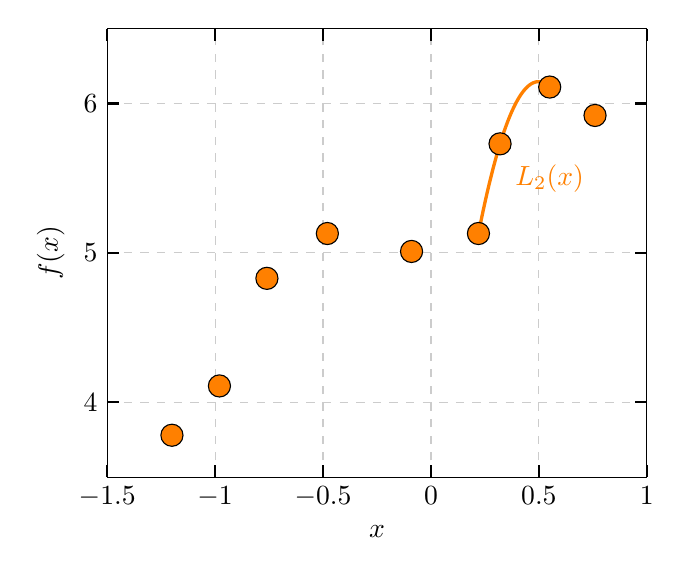
\begin{tikzpicture}
\begin{axis}[
xlabel = {$x$},		% подпись оси x
ylabel = {$f(x)$},	% подпись оси y
xmin=-1.5, xmax=1,
ymin=3.5, ymax=6.5,
xtick style={thick, black},
ytick style={thick, black},
grid=major,		
major grid style={color=black!20, dashed, thin},
]
\addplot[only marks, mark=*, mark size=4pt, mark options={fill=orange, draw=black, solid}] coordinates 
{(-1.2,3.78) (-0.98,4.11) (-0.76,4.83) (-0.48,5.13) (-0.09,5.01) (0.22,5.13) (0.32,5.73) (0.55,6.11) (0.76,5.92)};
\addplot[color=orange, very thick, samples=50, domain=0.22:0.55] {
-13.17523062*x^2+13.11462456*x+2.882463758
};
\draw[color=orange] (axis cs: 0.55,5.5) node {$L_2(x)$};
\end{axis}
\end{tikzpicture}
\end{figure}
% *******************************
Определим первую и вторую производную функции $y(x)$ в точке $x_6=0.32$:
\begin{gather*}
y^{\prime}(0.32)\approx L_2^{\prime}(0.32)=4.682476963\\
y^{\prime\prime}(0.32)\approx L_2^{\prime\prime}(0.32)=-26.35046124
\end{gather*}
% x7
\item
Апроксимацию функции $y(x)$ в узлах $\{x_{6},x_{7},x_{8}\}$
полиномом Лагранжа второго порядка $L_2(x)$, 
используя данные таблицы \ref{tab:Num_Diff}:
\begin{gather*}
\begin{matrix}
L_2(x)&=&
\dfrac{(x-0.55)(x-0.76)}{(0.32-0.55)(0.32-0.76)}\cdot5.73&+\\[1em]
&+&\dfrac{(x-0.32)(x-0.76)}{(0.55-0.32)(0.55-0.76)}\cdot6.11&+\\[1em]
&+&\dfrac{(x-0.32)(x-0.55)}{(0.76-0.32)(0.76-0.55)}\cdot5.92
\end{matrix}
\end{gather*}
Проводя элементарные алгебраические преобразования полином Лагранжа 
в пределах отрезка $[x_6,x_8]$ имеет вид:
\begin{gather*}
L_2(x)=-5.811217790\cdot x^2+6.707933391\cdot x+4.178530017
\end{gather*}
% *******************************
%	График функций
%
\begin{figure}[H]\centering
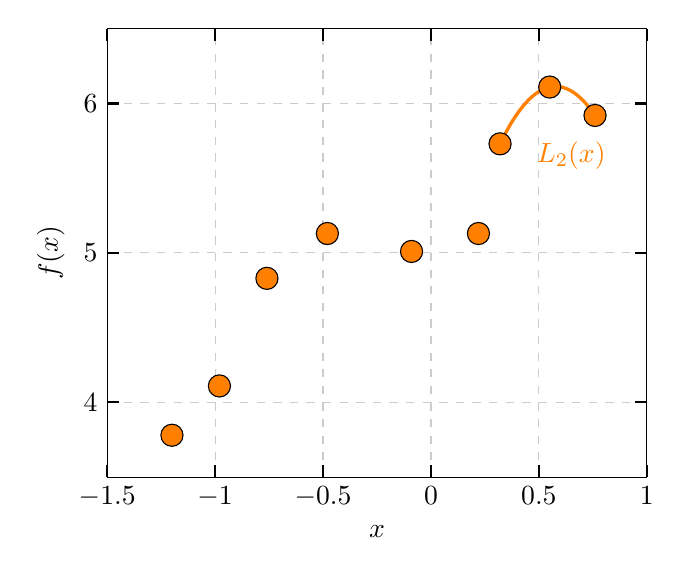
\begin{tikzpicture}
\begin{axis}[
xlabel = {$x$},		% подпись оси x
ylabel = {$f(x)$},	% подпись оси y
xmin=-1.5, xmax=1,
ymin=3.5, ymax=6.5,
xtick style={thick, black},
ytick style={thick, black},
grid=major,		
major grid style={color=black!20, dashed, thin},
]
\addplot[only marks, mark=*, mark size=4pt, mark options={fill=orange, draw=black, solid}] coordinates 
{(-1.2,3.78) (-0.98,4.11) (-0.76,4.83) (-0.48,5.13) (-0.09,5.01) (0.22,5.13) (0.32,5.73) (0.55,6.11) (0.76,5.92)};
\addplot[color=orange, very thick, samples=50, domain=0.32:0.76] {
-5.811217790*x^2+6.707933391*x+4.178530017
};
\draw[color=orange] (axis cs: 0.65,5.65) node {$L_2(x)$};
\end{axis}
\end{tikzpicture}
\end{figure}
% *******************************
Определим первую и вторую производную функции $y(x)$ в точке $x_7=0.55$:
\begin{gather*}
y^{\prime}(0.55)\approx L_2^{\prime}(0.55)=0.315593822\\
y^{\prime\prime}(0.55)\approx L_2^{\prime\prime}(0.55)=-11.62243558
\end{gather*}
\item
Таким образом, определены значения первой $y^{\prime}(x_i)$ и
второй $y^{\prime\prime}(x_i)$ производной функции $y(x)$ 
в каждом внутреннем узле сетки $\{x_i\}$:
\begin{center}
\begin{tabular}{ l *{7}{l}}
\toprule
$x$&-0,98&-0,76&-0,48&-0,09&0,22&0,32&0,55\\
\midrule
$f^{\prime}(x)$&2,39&2,30&0,50&0,08&4,63&4,68&0,32\\
\midrule
$f^{\prime\prime}(x)$&8,06&-8,81&-4,12&1,99&27,38&-26,35&-11,62\\
\bottomrule
\end{tabular} 
\end{center}
% *******************************
%	График функций
%
\begin{center}
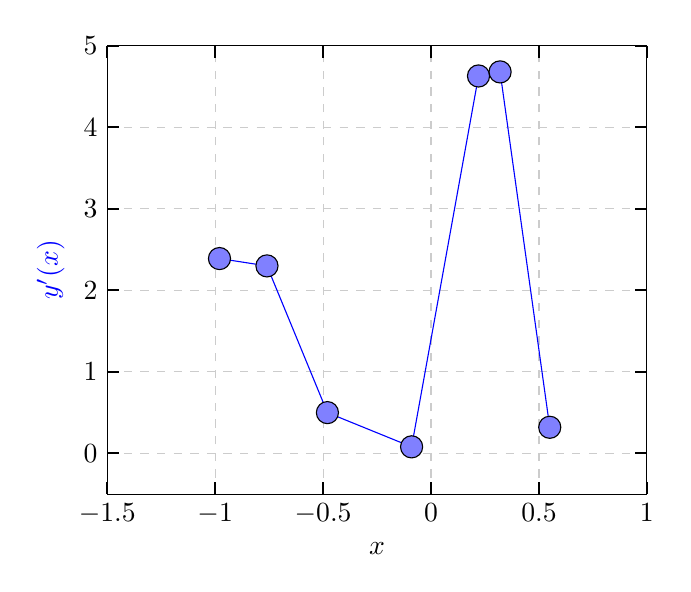
\begin{tikzpicture}
\begin{axis}[
xlabel = {$x$},		% подпись оси x
ylabel = {$\textcolor{blue}{y^{\prime}(x)}$},	% подпись оси y
xmin=-1.5, xmax=1,
ymin=-0.5, ymax=5,
xtick style={thick, black},
ytick style={thick, black},
grid=major,		
major grid style={color=black!20, dashed, thin},
]
\addplot[blue,mark=*, mark size=4pt, mark options={fill=blue!50, draw=black, solid}] coordinates 
{(-0.98,2.39) (-0.76,2.30) (-0.48,0.50) (-0.09,0.08) (0.22,4.63) (0.32,4.68) (0.55,0.32)};
\end{axis}
\end{tikzpicture}
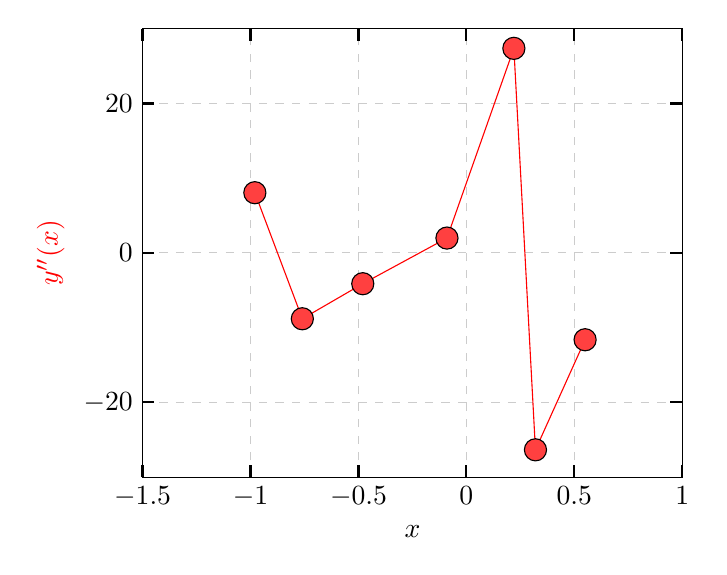
\begin{tikzpicture}
\begin{axis}[
xlabel = {$x$},		% подпись оси x
ylabel = {$\textcolor{red}{y^{\prime\prime}(x)}$},	% подпись оси y
xmin=-1.5, xmax=1,
ymin=-30, ymax=30,
xtick style={thick, black},
ytick style={thick, black},
grid=major,		
major grid style={color=black!20, dashed, thin},
]
\addplot[red,mark=*, mark size=4pt, mark options={fill=red!75, draw=black, solid}] coordinates 
{(-0.98,8.06) (-0.76,-8.81) (-0.48,-4.12) (-0.09,1.99) (0.22,27.38) (0.32,-26.35) (0.55,-11.62)};
\end{axis}
\end{tikzpicture}
\end{center}

\end{enumerate}

%\end{document}